\documentclass[11pt, a4paper]{report}

\usepackage [french, english]{babel}		% dire que l'on veut rédiger en français
\usepackage [utf8]{inputenc}		% dire que l'on veut utiliser tous les caractères du clavier
\usepackage [T1]{fontenc}		% dire que l'on veut utiliser tous les caractères du clavier
\usepackage {graphicx}
\usepackage [urlcolor=blue, colorlinks=true, linkcolor=blue]{hyperref}			% inclure pdf, png...
\usepackage {pdfpages}
\hypersetup {pageanchor=false}
\usepackage {geometry}
\geometry{hmargin=2.5cm, vmargin=2.5cm}

\title{Projet réseau S5 L3-I}
\author{Genevois / Thiercé / Ambrois / Chaumienne / Breton / Mahé}
\date{mars 2014}

\begin{document}

\maketitle
\renewcommand{\contentsname}{Sommaire}
\tableofcontents

\chapter{Introduction}

  \section{Contexte de réalisation}
    
    Ce projet a été réalisé dans le cadre du module réseau de L3 informatique de l'université de Cergy Pontoise. Il devait être réalisé 
    par une équipe de six personnes dont certaines avec des rôles précis :
    \newline
    
    \begin{itemize}
    
     \item Animateur et chef de projet : Thibaut Genevois
     \item Architecte technique : Nicolas Thiercé
     \item Secrétaire : Guillaume Ambrois
     \item Gardien du temps : Kévin Breton
     \item Scribe : Charles Chaumienne
     
    \end{itemize}
    
  \section{Sujet}
    
    L'objectif était de concevoir un jeu de type MMO basé sur une architecture client-serveur.
    \newline
    
    L'aspect important de ce projet est la robustesse des couches réseau. L'IHM peut être construite en ASCII, en 2D ou 3D, seuls les aspects tolérance
    aux pannes et performances réseau sont à développer consciencieusement.
    
  \section{Environnement technique}
    
    Les seules contraintes imposées en termes d’environnement technique sont les suivantes :
    \newline
    
    \begin{itemize}
    
     \item Client à écrire en Java SE
     \item Serveur à écrire en C
     
    \end{itemize}
    
\chapter{Spécifications}

  \section{Spécifications du jeu}
    
    Les fonctionnalités que nous avons définies pour le client sont les suivantes :
    
    \begin{itemize}
    
      \item S'authentifier
      \item Se déplacer sur la carte
      \item Se déconnecter\newline
	
    \end{itemize}
    
    Ces fonctionnalités sont très restreintes. Nous en avons décidé ainsi car notre objectif est de fournir une solution client-serveur robuste.\newline
    
    Le serveur acceptera un maximum de cent joueurs et la carte sera composée de quatre types de cases :
    \newline
    
    \begin{itemize}
    
      \item Rocher
      \item Herbe
      \item Eau
      \item Arbre\newline
	
    \end{itemize}
    
  \section{Spécifications de la couche réseau}
  
    \subsection{Protocole applicatif}
    
      Lorsqu'un joueur veut se connecter, il envoie une requête de connexion au serveur contenant son login et son mot de passe.
      Si le couple login/mot de passe existe et que le joueur n'est pas déjà connecté, le serveur lui envoie un paquet contenant 
      tous les noms et emplacement des joueurs connectés, sa position étant indiquée en premier.
      Sinon, le serveur lui envoie un paquet lui indiquant que la connexion n'a pas pu être effectuée.
      \newline

      Lorsqu'un joueur veut se déplacer, une requête est envoyée au serveur, qui détermine si le déplacement est valide.
      S'il l'est, le serveur envoie un paquet à tous les clients indiquant que le joueur s'est déplacé.
      Sinon, le serveur envoie un paquet seulement au joueur ayant effectué le déplacement, lui signifiant que son déplacement 
      a été refusé.
      \newline

      Lorsqu'un joueur veut se déconnecter, il envoie une requête de déconnexion au serveur, qui sauvegarde sa position et envoie 
      un paquet à tous les joueurs présents sur la carte, leur indiquant que le joueur s'est déconnecté.
      \newline

      Des requêtes de ping sont effectuées régulièrement par des clients afin de vérifier que le serveur est toujours accessible.
      Des requêtes de ping sont également effectuées régulièrement par le serveur pour s'assurer que tous les clients sont toujours 
      connectés.
    
    \subsection{Les paquets}
    
      La section précédente expose les différentes données échangées entre le serveur et un ou plusieurs clients.
      \newline
      
      Ces données sont de tailles très différentes selon leur type. Par exemple, lorsque le client envoie une demande d'authentification au serveur, les données envoyées sont le pseudo et 
      le mot de passe (soit une longueur totale oscillant entre 10 et 40 caractères).
      Cependant, quand le serveur renvoie au client le refus de la demande d'authentification, un octet suffit (car, pour des raisons de sécurité, on ne notifie pas la raison de ce refus au client).
      De plus, transmettre en représentation binaire de certains types de données (au lieu d'une représentation en chaine de caractères), tels que les nombre entiers, permettrait de réduire la taille
      de ces dernières.
      \newline
      
      Par conséquent, un système de paquets encapsulant les données échangées est mis en place, afin de détecter de façon homogène le début et la fin de chaque séquence de données.
      Ce dernier point est indispensable si le flux entrant contient plusieurs messages en attente d'être traité.
      \newline
      
      Chaque paquet est composé d'un entête et d'un champ de données. Ce dernier est de taille variable et peut être vide.
      L'entête contient 3 champs : l'identifiant de début de paquet, la longueur des données et le type de paquet. Le champ identifiant de début de paquet, un entier signé sur 32 bits,
      sert à détecter le début de chaque paquet reçu.
      Le champ longueur des données est un entier sur 32 bits qui représente la taille du champ de données en octets.
      Le champ type est un entier signé sur 8 bits, et permet de rapidement décider de l'action à réaliser.
      Par exemple, si le client reçoit un paquet de type 2, il déclenche l'action correspondante au refus de demande d'authentification.
      \newline
      
      Comme le serveur est composé deux services, à chacun de ces services est associé une plage de valeurs pour le champ type de données (le découpage de cette plage 
      est analogue au celui d'une plage d'adresses IP).
      Cela permet de savoir rapidement à quel service correspond un paquet, en utilisant une condition d'égalité et un "et" binaire.
      Le service authentification a la plage de valeurs 0-31 et le service jeu gère les valeurs de l'ensemble 32-63.
      \newline
      
      Le tableau ci-dessous spécifie, pour chaque type de communication, la valeur du champ type, le sens d'envoi ("client -> serveur" ou "serveur -> client"), ainsi 
      que le format du champ de données correspondants.

      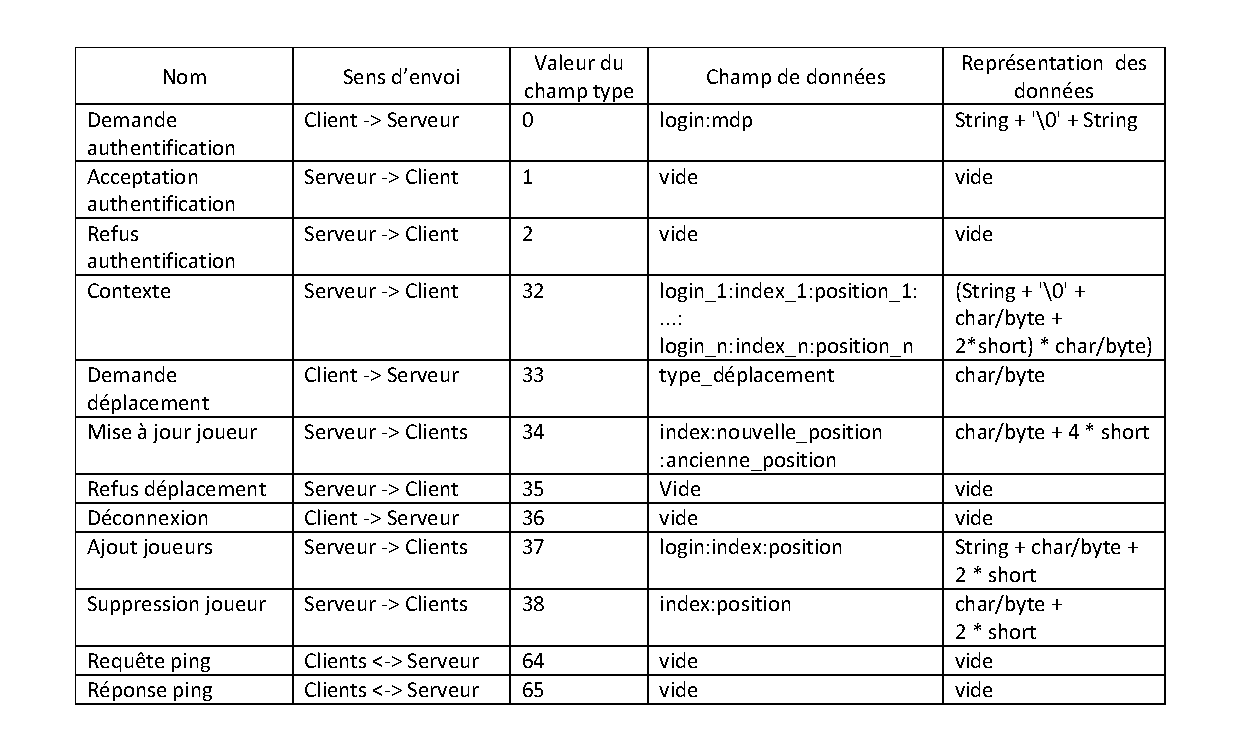
\includepdf{tableau_paquets.pdf}
      
      Note : ici, le type String représente une suite de caractères au format ascii (seuls les caractères de la table ascii non étendue sont utilisés). 
    
    \subsection{Protocole réseau sous-jacent}
    
      Le protocole applicatif ne permettant pas la perte de données, les communications réseaux doivent être fiables et en mode connecté.
      Par conséquent, le protocole réseau sous-jacent à utiliser est TCP (Transmission Control Protocol).
      \newline
      
      Afin d'éviter la congestion du réseau, ce dernier accumule les données à envoyer jusqu'à une certaine quantité d'octets ou pendant un certain temps, 
      puis les envoie dans un seul paquet (comportement par défaut). Cependant, comme le projet réalisé nécessite du temps réel et principalement des 
      échanges de données de l'ordre de 20 octets, ce comportement sera désactivé (par le biais de l'option TCP\_NO\_DELAY) afin d’accroître les performances.
	  
    \subsection{Gestion des erreurs}
    
      \subsubsection{La perte de connexion}
    
	Tcp est un protocole de communication en mode connecté, c'est pourquoi si un paquet envoyé n'est pas transmis 
	(acquittement correspondant non reçu) dans un certain délai (ou time-out), la connexion est considérée comme perdue.
	\newline
      
	Cependant, par défaut, ce problème n'est pas géré lorsqu'il n'y a aucun trafic réseau. Donc, pour pallier à ce problème, il existe l'option TCP\_KEEP\_ALIVE. 
	Cette dernière active le comportement suivant : après un certain temps h d'inactivité (par défaut, h = 2 heures), un paquet tcp ayant le rôle d'un "ping" 
	est envoyé et une réponse immédiate est demandée; si aucune "réponse" n'est reçue au bout de t secondes (par défaut, t=75), cette opération est de nouveau 
	effectuée.
Si au bout de n tentatives (par défaut, n=9), aucune réponse n'est reçue, la connexion est considérée comme perdue. Donc, par défaut, 
	une connexion peut être considérée comme perdue après 2*3600 + 75*9 = 7875 secondes, soit environ 2 heures et 11 minutes.
	\newline
	
	Ce temps de détection n'étant pas acceptable pour un jeu multi-joueurs en réseau, et les délais n'étant pas modifiables en java, l'utilisation de cette 
	option a été abandonnée. La solution finalement retenue est l'envoi, après un certain temps d'inactivité de 1 seconde, d'un paquet de type "demande ping";
	afin de relancer l'activité sur la connexion. Donc, la perte de connexion est bien détectée. Ensuite, l'application cliente et le serveur gèrent en conséquence.
	\newline
      
      \subsubsection{Identification du début des paquets reçus}
      
	Supposons que l'on réceptionne dans le flux entrant de la connexion un paquet de 16 octets avec une longueur des données erronée, par exemple 8 octets 
	au lieu de 11. Dans ce cas, l'entête du paquet reçu est extraite du flux et analysée, puis les 8 octets du champ de données sont retirés. Il reste donc
	3 octets dans le flux. Si un autre paquet est reçu pendant l'opération précédente, ce dernier ne sera pas lu correctement puisque l'entête qui sera analysée 
	contiendra les 3 octets restants du paquet précédent. Par conséquent, le champ "taille des données" peut contenir la valeur 100 000 au lieu de 1 octet,
	et ce paquet n'aura plus de sens.
	\newline
	
	Afin de pallier à ce problème, il y a un champ "identifiant" au début de l'entête des paquets (ce dernier a une valeur fixe sur 32 bits). 
	Pour détecter le début du paquet, l'algorithme suivant est utilisé :
	\newpage
	\indent TANT qu'il reste au moins 4 octets à lire dans le flux FAIRE\\
	  \indent\indent lire ces 4 premiers octets\\
	  \indent\indent SI ils correspondent à la valeur fixée précédemment\\
	    \indent\indent\indent lire le paquet\\
	    \indent\indent\indent sortir de la boucle\\
	  \indent\indent SINON\\
	    \indent\indent\indent retirer 1 octet du flux\\
	  \indent\indent FIN SI\\
	\indent FIN TANT QUE\\
    
\chapter{Implémentation}
  
  \section{Client}
  
    \subsection{GUI}

Avant de parler de la constitution de l'interface graphique, je vous propose de visualiser le résultat. La première figure vous dévoile la page de connexion. Un formulaire de connexion on ne peut plus simple mais entièrement fonctionnel.
La seconde, vous montre le jeux avec deux personnages de connecté. L'un est le nôtre, devinerez-vous lequel?

\begin{figure}[!ht]
   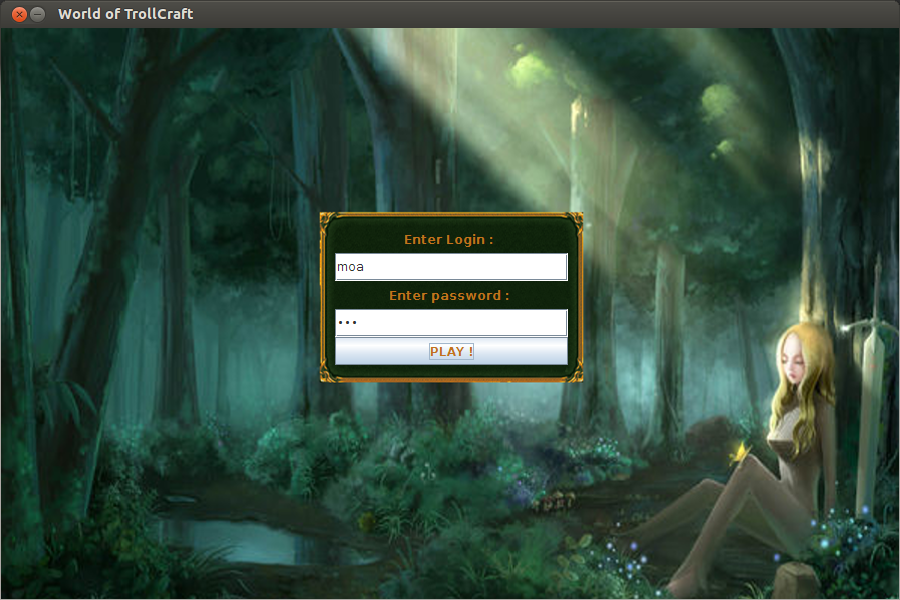
\includegraphics[width=16cm]{page_connexion.png}
   \caption{Ecran de connexion}
\end{figure}

\begin{figure}[!ht]
   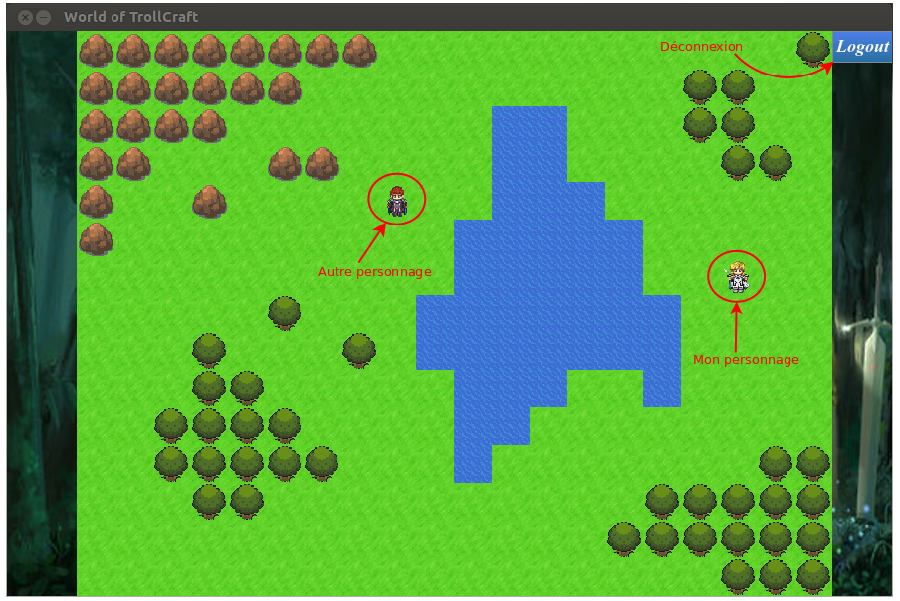
\includegraphics[width=16cm]{game.png}
   \caption{Deux personnages en jeu}
\end{figure}

\newpage
\subsubsection{Structure de l'interface}

\paragraph{Le JLayeredPane}


L'interface de cette application a été fondée sur un système de couches de textures. Il a donc été nécessaire de rechercher quel objet avait la possibilité de contenir une multitude de \verb{JPanel{ et de les afficher selon l'ordre que le développeur aurait choisi. Il s'agit de la classe \verb{JLayeredPane{.
Nous avons donc dans un premier temps, implémenté une interface graphique basique sur laquelle nous avons défini un \verb{JlayeredPane{ comme \verb{ContentPane{ de la fenêtre. Ainsi, nous pouvons désormais contenir l'ensemble des couches de textures, qui seront nécessaires à la construction et au bon fonctionnement de cette interface.

\paragraph{Les JPanel(s)}

Les \verb{JPanel{ qui constituent cette interface sont principalement au nombre de cinq :
\begin{itemize}
\item \verb{connexion{
\item \verb{formulaire{ 
\item \verb{tacticPanel{ 
\item \verb{texturePanel{
\item \verb{playerTexture{
\end{itemize}

\subparagraph{Page de connexion}

Le \verb{JPanel{ \verb{Connexion{ ne contient que l'image de fond visible lors du démarrage de l'application. C'est aussi sur cette image que l'on a dessiné le cadre contenant le formulaire de connexion.
\verb{formulaire{ est un \verb{Jpanel{ dont le \verb{Layout{ a été instancié à l'aide d'un \verb{GridLayout{ pour la mise en forme du formulaire. Ce \verb{JPanel{ a été redimensionné de manière à faire coïncider parfaitement avec le cadre dessiné sur l'image de connexion. De plus, \verb{formulaire{ s'est vu attribuer un statut de transparence pour un rendu homogène de la page de connexion.
\verb{JLayeredPane{ permet d'ajouter des \verb{JPanel{ les un au-dessus des autres selon un indexage précis allant de 1 à -n, nous avons donc superposé ces deux \verb{JPanel{ le plus "au-dessus" possible de manière à placer la page de connexion au premier plan de l'application.

\subparagraph{Textures de Map}

L'affichage de la \verb{Map{ sera confié à un \verb{JPanel{. Celui-ci aura pour but de fournir un affichage complet des textures. Nous verrons par la suite comment nous remplirons ce \verb{JPanel{ d'affichage, mais sachez qu'il est définit en tant que \verb{GridLayout{ au nombre de case en largeur et en hauteur de la map.
Chaque cellule de ce \verb{JPanel{ sera remplie avec un jeu d'objet dérivant de la classe \verb{JPanel{ adapté à chaque texture. On retrouve pour les textures les classes suivantes :
\begin{itemize}
\item \verb{GrassTesture{ : représentation de l'herbe
\item \verb{RockTexture{ : représentation des rochers
\item \verb{WaterTexture{ : représentation de l'eau
\item \verb{TreeTexture{ : représentation des arbres			
\end{itemize}

\paragraph{Texture de Joueurs}

En ce qui concerne les textures des personnages du jeu, on en compte deux. La première sera la représentation de notre personnage. La seconde sera celle appliquée à tous les autres personnages présents sur la carte. On notera que le personnage est représenté par un jeu de quatre images de textures. Une pour chaque direction dans laquelle le personnage est censé se déplacer.
La particularité des textures de joueurs est qu'il ne s'agit pas de \verb{JPanel{. Ici nous avons utilisé des objets de type \verb{Image{ que nous dessinerons sur le contexte graphique grâce à la méthode \verb{drawImage(){ aux coordonnées du personnage.

\subsubsection{Fonctionnement de l'interface}

\paragraph{L'initialisation de l'interface graphique}

\subparagraph{La construction de la map}

L'interface graphique avant même d'apparaître doit être apte à offrir à l'utilisateur toutes les informations. On va dons dans un premier temps instancier un objet de type \verb{Manager{ dans le but de récupérer la grille afin de l'interpréter et de l'afficher. On récupère donc ses dimensions. Il se pose alors un problème. L'idée est de générer une fenêtre de taille fixe mais pour une grille d'une taille infinie. Il faut donc trouver la taille en pixel des cellules de la grille sachant qu'elles doivent être carré, car représentée par des images de textures de 64 par 64 pixels. Pour cela, nous avons alors implémentés un algorithme qui effectue les actions suivantes : On va dans un premier temps savoir si la largeur estimé est plus grande que celle de la fenetre. Si ce n'est pas le cas, on regarde en fonction de la hauteur. Si la hauteur estimé dépasse celle de la fenetre, on recalcule le coté de la case en fonction de la hauteur. Sinon les images dans leurs tailles orginiales rentrerons dans la fenêtre. 
Sans trop détailler, nous allons discrétiser les cas possible et calculer le coté d'une case en fonction soit de la hauteur soit de la largeur.
L'étape suivante sera de calculer la position de la grille dans la fenêtre afin de la centrer.
Une fois le coté de la case déterminé, on peut interpréter la grille et affecter une texture a chaques cellules lues. Pour cela on fera appels au méthodes \verb{add...Texture(){.
On ajoute alors le panel de la map au \verb{ContentPane{ de la fenêtre.

\subparagraph{La page de connexion}

La page de connexion se base sur deux \verb{JPanel{ un pour afficher l'image de fond qui dissimulera la map texturé déjà présente et un autre pour le formulaire de connxexion.
Pour l'image de fond nous ferons appel a un objet dérivé de \verb{JPanel{ qui sera \verb{ConnexionTexture{. Ne nous reste alors qu'a créer un \verb{JPanel{ formulaire de layout \verb{GridLayout{ pour contenir les labels les champs de saisies et le bouton de validation.

\subparagraph{La méthode update}

La méthode \verb{update(){ est sans doute un élément nécessaire au bon fonctionnement de cette interface. Cette méthode lit les paquets reçu par le client, et offre une interprétation pour chacun de ces paquets. Ainsi, nous retrouvons les actions à effectuer, qu'il s'agisse d'une connexion de notre part ou non, d'un déplacement ou encore d'une déconnexion. On notera aussi que le refus de connexion par le serveur a aussi été traité par l'affichage d'une boîte de dialogue dont la particularité est qu'elle ne dévoile pas le contenu de l'erreur. 

\paragraph{Connexion, déconnexion et déplacements}

\subparagraph{La connexion}

 Le mécanisme de connexion passe d'abord par l'action effectuée lors de l'appui sur le bouton de connexion. On va donc vérifier l'intégrité des différents champs du formulaire de connexion ainsi que l'accessibilité du serveur. Une fois la requête envoyée, la fonction \verb{update(){ interprète la réponse du serveur. Les panels de connexion sont alors supprimé et laissent place à la map. Les joueurs eux sont ajouté en parallèle puisque le serveur a envoyé en réalité deux message.
On appelle donc la méthode \verb{displayPlayers(){ qui se chargera de lire la hashmap des joueurs connectés et de les dessiner sur un \verb{JPanel{ placé sur une couche du \verb{JLayeredPane{. On appelle alors une méthode pour ajouter le bouton de déconnexion.
Lors de la connexion d'un nouveau joueur lors de notre présence sur le jeu, un traitement spécifique a été mis en place dans la méthode \verb{update(){ qui va rafraîchir le panel \verb{PlayerTexture{. Ceci aura pour effet de dessiner un joueur en plus à ses coordonnées.

\subparagraph{Les déplacements}

Les déplacement se décomposent en deux cas, le premier est la demande de déplacement, la seconde est l'autorisation. La demande s'effectue à l'aide des \verb{Listener{ mis en place sur les flèches du clavier. Une requête est alors envoyée au serveur via le client.
Dans le cas d'un déplacement validé par le serveur la réponse est traitée par la méthode \verb{update(){. On transmet alors au \verb{PlayerTexture{ les diverses informations nécessaire à la mise à jour de ce panel. Ainsi, on va dans un premier temps détecter s'il s'agit de notre personnage ou celui d'un autre dans le but d'attribuer la texture associée. On redessine alors une texture de \verb{Grass{ à la position de l'ancienne coordonnée et la texture asssociée à la direction à la nouvelle coordonnée.
\subparagraph{La déconnexion}

Lors de la déconnexion d'un joueur, un rafraîchissement de la couche joueur est appellée ce qui entraîne l'application de la texture d'herbe sur ses coordonnées. En revanche lors d'une déconnexion intempestive ou lors de l'appuis sur le bouton mis à disposition, on fait appel à la méthode \verb{disconnection(){. Celle-ci fermera le client et l'envoie de données. Le bouton de déconnexion est alors retiré et on réinstancié les panels de la page de connexion.

\subsubsection{Evolution possible de l'IHM}
 
Il est vrai que cette interface est fonctionnelle. On notera l'utilisation d'un double buffer pour améliorer ses performances de rafrîchissement demandées lors de déplacements. En revanche des améliorations sont possibles. On pourrait imaginer par exemple que lorsque l'authentification est réussie on appelle une autre frame, ce qui nous permetterait de charger les données plus efficacement mais aussi rendrai plus efficace la protection du reste de l'application.
Des textures plus dynamiques peuvent être aussi envisagées. D'autres améliorations tels qu'un canal de discussion on un impact à un niveau bien plus bas que l'IHM et ne seront pas présentées ici.
    
    \subsection{Couche réseau}
    
      Il n'y a qu'une seule classe utilisée pour la couche réseau, il s'agit de la classe Client.
      \newline
      
      Elle a comme attributs :
      
      \begin{itemize}
      
	\item Les constantes identifiant les différents types de paquet
	\item L'en tête des paquets
	\item Le port et l'adresse IP du serveur, qui sont lues à partir d'un fichier de configuration
	\item Un Socket relié au serveur
	\item BufferedInputStream et BufferedOutputStream pour pouvoir dialoguer avec le serveur (en flux, par TCP)
	\item Une référence vers le Manager, classe principale du moteur
	\item Un Timer qui, une fois la connexion avec le serveur effectuée, envoie des requêtes de type "Ping" toutes 
		      les secondes pour vérifier si la connexion entre le serveur et le client existe toujours\newline	
      \end{itemize}
	
      Lors de l'initialisation, si la connexion entre le serveur et le client s'établit, un nouveau Thread d'écoute est lancé.
      Son seul rôle est de lire en permanence le flux d'entrée, et si des données sont reçues, vérifier si le champ d'en tête est 
      valide. Si ce dernier est valide, le Thread extrait les données de la trame et les envoie au Manager pour qu'il traite 
      les informations.
      \newline
      
      La classe dispose également d'une méthode permettant de fermer la connexion entre le serveur et le client, 
      en fermant les flux d'entrée et de sortie, puis en fermant le Socket.
      \newline
      
      Enfin, la méthode sendData() permet d'envoyer les données vers le serveur. Elle reçoit les données à envoyer sous forme 
      de tableau de Byte ainsi que la longueur du paquet à envoyer, et envoie le paquet au serveur.
      \newline
      
      Evidemment, toutes les exceptions sont gérées et des logs sont générés pour chaque action.
    
    \subsection{Moteur}
    
      Le fichier GameClient.properties contient le port et l'adresse du serveur, log4j.properties contient la configuration des logs
      et standard\_map.txt contient la représentation textuelle de la carte.
      \newline
      
      La seule bibliothèque externe utilisée dans ce projet est log4j (génération de fichiers de log).
      \newline
      
      Il existe 2 énumérations, une représentant les types de décor (SetType), et l'autre représentant les directions 
      de déplacement possibles (Direction).
      \newline
      
      La surface de jeu est représentée par l'instanciation de la classe Map. Celle-ci dispose de plusieurs attributs :
      
      \begin{itemize}
\item La taille maximale de la carte (en hauteur et en largeur, fixées respectivement à 75 et 100)
\item La taille effective de la carte
\item Une HashMap de joueurs connectés, indexés par leur index
\item Une référence vers le joueur local
\item Un tableau à 2 dimensions d'objets de type Cell, représentant une case de la carte
      \end{itemize}
      
      Lors de l'initialisation de la carte, le fichier "standard\_map.txt" est lu et interprété, ce qui remplit le tableau 
      représentant la carte. Le fichier contenant la carte doit évidemment être bien formé, ce qui est vérifié grâce à 
      l'utilisation de la méthode match() et une expression régulière décrivant le fichier tel qu'il devrait être.
      \newline
      
      La surface de jeu étant représentée par une grille, une classe Coordinate a été utilisée afin de pouvoir désigner 
      chacune des cases de la grille, et de pouvoir les comparer entre elles ou faire des opérations 
      (translation dans une direction, position relative de 2 cases).
      \newline
      
      Les classes Player et Set, qui représentent respectivement un joueur et du décor, étendent toutes les deux la classe 
      abstraite Cell, qui ne dispose que d'une méthode renvoyant le type d'élément de l'objet 
      (0 si c'est un joueur, 1 si c'est un décor, 2 si la case est libre).
      \newline
      
      Il existe 3 types de décor "obstacles", avec les mêmes propriétés (seul l'aspect visuel change) :
      
      \begin{itemize}
    
	\item Les rochers
	\item Les arbres
	\item L'eau
	
      \end{itemize}

      Chacun de ces décors représente un obstacle pour les joueurs. Ils ne peuvent pas les traverser mais ces décors ne
      gênent toutefois pas la vision.
      \newline
      
      Les joueurs présents sur la grille sont des instanciations de la classe Player, qui ne dispose que de 3 attributs :
      \begin{itemize}
\item Le pseudo du joueur
\item L'index du joueur (son identifiant unique)
\item Ses coordonnées
\end{itemize}
      
      Le but du projet étant de mettre en pratique les différents protocoles réseaux, et non de réaliser un jeu, 
      nous n'avons pas jugé utile de développer le côté "RPG" de l'application. C'est pourquoi un joueur ne dispose pas 
      de points de vie, de points de mana ou autres attributs relatifs à un personnage de RPG.
      \newline
      
      Enfin, c'est dans la classe Manager que se passent tous les traitements, que ce soit les données reçues du serveur 
      et extraites par la classe Client, ou les différentes actions du joueur local.
      \newline
      
      A la création du Manager, la construction de la Map est lancée.
      \newline
      
      Lors de l'initialisation, qui correspond au moment où l'utilisateur essaye de se connecter, un objet Client est 
      instancié et initialisé.
      \newline
      
      C'est dans cette classe que les paquets extraits par le Thread d'écoute de la classe Client sont traités dans la méthode 
      paquetOpeningFactory(). En fonction du type du paquet, des traitements seront effectués. Par exemple, si le type du paquet
      est 1, c'est une réponse positive du serveur à la demande de connexion de l'utilisateur. Si le type du paquet est 34, cela 
      veut dire qu'un joueur s'est déplacé, et le paquet contient l'index du joueur qui a bougé ainsi que son ancienne et 
      nouvelle coordonnée.
      \newline
      
      Les méthodes "dataObserver..." permettent ensuite de communiquer à l'IHM, via la méthode setData(), les données traitées,
      grâce à un design pattern Observable/Observer.
      \newline
      
      Le Manager dispose de 3 méthodes :
      \begin{itemize}
\item sendDataLogin() qui envoie les identifiants de l'utilisateur au serveur dans une requête de connexion
\item sendDataMove() qui envoie une requête de déplacement dans la direction fournie au serveur
\item sendDataLogout() qui indique au serveur que l'utilisateur s'est déconnecté
\end{itemize}
      
      Cette méthode est appelée par la méthode logout(), qui fait ensuite appel à la méthode closeClient() du Client 
      pour fermer les flux et le Socket en plus de prévenir le serveur de la déconnexion.
      Chacune de ces méthodes fait appel à la méthode sendData() du Client, en lui fournissant un tableau de données 
      et la longueur du champ de données.
      
  \section{Serveur}
  
    \subsection{Moteur}
    
      Le moteur travail principalement avec une file des joueurs en attente d'être placés sur la carte, une file de joueurs devant être 
      éjectés de la carte (perte de connexion, a simplement quitté le jeu), une carte 'du monde' (chargée depuis un fichier texte) et des joueurs.
      \newline
      
      La carte du monde est représentée par une structure WorldMap ayant :
      \newline
      
      \begin{itemize}
	\item Une longueur et une largeur
	\item Un tableau à deux dimensions de cellules (Cell)
	\item Une structure de type PlayerManagement\newline
      \end{itemize}
      
      La structure PlayerManagement est une structure de gestion des joueurs, elle permet de savoir combien de joueurs sont actuellement sur la carte
      et maintient un tableau de ces derniers. Cette structure est composée des éléments suivants :
      \newline

      \begin{itemize}
	\item Un tableau de joueurs
	\item Une pile des index du tableau qui sont libres et peuvent être utilisés
	\item Un entier représentant le nombre de joueurs présents sur la carte\newline
      \end{itemize}
    
      Une cellule (Cell) est une union qui représentera soit un décor, soit une case avec un joueur :
      \newline
      
      \begin{itemize}
	\item Un entier représentant le type de l'union
	\item Une case de décor (SetCell)
	\item Une case joueur (Player Cell)\newline
      \end{itemize}
      
      Une case de décor (SetCell) contient une énumération pour définir le décor. Une case joueur (Player Cell) contient un structure de type Player.
      \newline
      
      Enfin, une structure joueur (Player) est composée des élements suivants :
      \newline

      \begin{itemize}
	\item Un entier représentant l'index de l'objet Player dans le tableau de PlayerManagement
	\item Une structure pour conserver la position du joueur sur la matrice carte (Position)
	\item Une chaine de caractères pour le login
	\item Une structure regroupant ce qui concerne la couche réseau (Connection)\newline
      \end{itemize}
      
      Le moteur a pour objectif de fédérer les interactions entre les joueurs et la carte car le client java ne dispose que d'une copie de cette dernière
      avec les décors.
      \newline
      
      Le moteur construit tout d'abord la carte de jeu à partir d'un fichier texte, dont il va vérifier la bonne syntaxe, puis placer au fur et à mesure des 
      authentifications réussis les joueurs sur la carte. Ces derniers se verront attribué une position aléatoire si c'est la première fois qu'ils se connectent
      ou seront placés sur leur dernière position connu si elle est libre.
      \newline
      
      Le moteur est le seul à savoir ce qui se trouve sur la matrice de cellules. Il gère donc les ajouts / suppressions de joueurs (déconnexion volontaire ou
      perte de contact avec le client) sur la carte et informe tout autre client sur la carte des modifications de positions qui ont eu lieu.
      \newline
      
    \subsection{Couche réseau}
  
  \chapter{Phase de test}
  
      \section{Presentation du protocole de test}
	
	Afin d'éprouver la solidité du serveur nous avons modifié le programme client. Une fois l'étape d'authentification
	passée, le client rentre dans une boucle infinie de déplacements aléatoires sur la carte.
	\newline
	
	Ce protocole de test a été mise en place et effectué sur les postes de l'université dans la salle B532 (dix postes exécutants des clients Java et 
	un poste exécutant le serveur).
	Les postes possèdent les caractéristiques suivantes :
	\newline
	
	\begin{itemize}
	  \item Intel Core 2 duo E6550 2,33 GHz
	  \item 2 Go PC2-6400
	  \item Carte réseau Gigabit
	  \item Ubuntu 12.04 64 bits
	\end{itemize}

      \section{Analyse des résultats}
	
	Sur le poste exécutant le serveur, la carte réseau affiche 50ko/s en réception et 250ko/s en émission. De plus, le processeur indique 50\% 
	d'utilisation un total de 140 ko de mémoire vive est consommé.

  \chapter{Analyse critique}

    \section{Points forts}
    
      \begin{itemize}
      
       \item Les paquets du jeu étant identifiés par un champ entête unique, codé sur 4 octets, les possibilités d'injecter des données et de tricher dans le jeu
	      sont restreintes.\newline
	\item Le serveur est relativement stable et performant car il consomme peu de ressources même en condition de stress test.\newline
	\item Le programme serveur est capable de détecter la perte de connexion avec un client et d'agir en conséquence vis à vis de l'avatar virtuel du joueur 
	      sur la carte.\newline
       
      \end{itemize}

    \section{Points faibles}
    
      \begin{itemize}
      
	\item Lorsque le programme serveur bug soudainement, les clients ne reçoivent pas le signal de déconnexion.\newline
	\item Lorsqu'un client est brutalement déconnecté, le serveur tente toujours de lui envoyer des paquets\newline
	\item Client ne disposant d'aucune fonctionnalité de jeu\newline
	\item Le traffic réseau n'est pas chiffré. Les mots de passes passent en clair\newline
	
      \end{itemize}
      
    \section{Améliorations possibles}
    
      \subsection{Client}
      
	\begin{itemize}
      
	  \item Correction d'un bug de l'interface graphique côté client qui n'efface pas les personnages lors d'une déconnexion\newline
	  \item Modification des méthodes d'affichage du client (taux de raffraîchissement fixe plutôt que raffraîchir à chaque paquet reçu)\newline
	  
	\end{itemize}

      \subsection{Serveur}

	\begin{itemize}
      
	  \item Améliorer la sécurité (chiffrer les données, déconnecter un spammeur)\newline
	  \item Ajouter la possibilité de piloter le serveur (arrêt propre, redémarrage, réinitialisation, ...)\newline
	  
	\end{itemize}
	
      \subsection{Globale}
      
	Une grande amélioration possible serait d'ajouter des fonctionnalités au jeu qui sont actuellement très restreintes.
      
\chapter{Organisation interne}      

  \section{Phase de spécifications}
  
    Tous les membres du groupe ont participé à la phase de spécifications. Celle-ci a consisté en une série de réunions où toutes les spécifications du 
    client et du serveur ont étés pensées et approuvées par l'ensemble du groupe.
    \newline
  
  \section{Répartition des taches}
  
    Concernant la phase d'implémentation les tâches ont été répartis comme suit :
    \newline
  
    Serveur :
    \begin{itemize}
      
	\item Moteur : Thibaut Genevois
	\item Couche Réseau et gestion de comptes : Nicolas Thiercé\newline
	
    \end{itemize}
    
    Client :
    \begin{itemize}
      
	\item Moteur et couche réseau : Guillaume Ambrois
	\item IHM : Charles Chaumienne et Kévin Breton\newline
	
    \end{itemize}

\chapter{Conclusion}

  \section{Difficultés rencontrées}
  
    Les premières difficultés rencontrées ont été de l'ordre de l'organisation interne du groupe, en particulier lors des séances de travail 
    collectif ou des réunions :
    
    \begin{itemize}
    
	  \item Respect et écoute du collègue qui parle
	  \item Synthétiser sa pensée
	  \item Respect des délais pour implémenter
	  
    \end{itemize}
    
    D'un point de vue technique, une difficulté que nous avons rencontré et surmonté concernait l'échange de nombres entiers entre le serveur et le client.
    En effet, il est nécessaire en C de convertir via les fonctions htonl (host to network long) et ntohl (network to host long) les entiers que l'on transmet via 
    le réseau. Ces conversions sont automatiques en Java. Nos programmes clients et serveurs 'ne parlaient pas la même langue' à un moment donné pendant les phases
    d'implémentation.
  
  \section{Ce que nous avons appris}
  
    D'un point de vue technique nous avons appris à programmer des logiciels capables de communiquer dans le cadre d'une architecture client-serveur.
    L'indépendance des couches réseau vis à vis de l'environnement technique a été mise en avant car nos deux logiciels client et serveur ont été programmés
    dans des langages bien différents.
    \newline
    
    D'un point de vue humain à présent, ce projet a été le premier à nous plonger dans le monde du travail collaboratif par groupes de plus de deux personnes.
    Il n'a pas été aisé d'apprendre à travailler ensemble. Nous y sommes tout de même parvenus, parfois au prix de séances inefficaces où les batailles d’ego 
    faisaient rage. Nous nous sommes ainsi quelque peu rapprochés de l'objectif final : savoir adopter un comportement professionnel dans le cadre de projets
    informatiques.
  
\chapter{Annexe}

  \href{http://tldp.org/HOWTO/TCP-Keepalive-HOWTO/index.html}{Description du mode tcp keep alive}\newline
  \begin{itemize}
    
    \item TCP/IP : architectures, protocoles et applications de Douglas Comer, 5ème édition, Pearson éducation
    
  \end{itemize}

\end{document}
